\documentclass{article}
\usepackage[utf8]{inputenc}
\usepackage[margin = 1 in]{geometry}
\usepackage{listings}
\usepackage{xcolor}
\usepackage{booktabs}
\usepackage{graphicx}


\definecolor{codegreen}{rgb}{0, 0.6, 0}
\definecolor{codegray}{rgb}{0.5, 0.5, 0.5}
\definecolor{codepurple}{rgb}{0.58, 0, 0.82}
\definecolor{backcolour}{rgb}{0.95, 0.95, 0.92}

\lstdefinestyle{mystyle}
{
	backgroundcolor =\color{backcolour},
	commentstyle =\color{codegreen},
	keywordstyle =\color{magenta},
	numberstyle =\tiny\color{codegray},
	stringstyle =\color{codepurple},
	basicstyle =\ttfamily\footnotesize,
	breakatwhitespace = false,
	breaklines = true,
	captionpos = b,
	keepspaces = true,
	numbers = left,
	numbersep = 5pt,
	showspaces = false,
	showstringspaces = false,
	showtabs = false,
	tabsize = 2
}

\lstset{style = mystyle}
\begin{document}
\begin{titlepage} % Suppresses displaying the page number on the title page and the subsequent page counts as page 1

\raggedleft\rule{1pt}{\textheight} % Vertical line
\hspace{0.05\textwidth} % Whitespace between the vertical line and title page text
\parbox[b]{0.75\textwidth}
	{% Paragraph box for holding the title page text, adjust the width to move the title page left or right on the page

            {\Huge\bfseries MIT World Peace University \\[0.5\baselineskip] \ SET}\\[2\baselineskip] % Title
            {\large\textit{Assignment 6}}\\[4\baselineskip] % Subtitle or further description
            {\Large\textsc{Naman Soni Roll No. 10}} % Author name, lower case for consistent small caps

   \vspace{0.5\textheight} % Whitespace between the title block and the publisher
   }

\end{titlepage}
\tableofcontents
\pagebreak
\section{\textbf{Aim}}
Object Oriented Analysis and design using UML diagrams: Sequence diagram to show message exchanges, using Open Source Tool.
\section{\textbf{Objectives}}
\begin{itemize}
    \item To learn the relationships and notions of Activity Diagram.
    \item To learn the relationships and notation of state chart diagram.
\end{itemize}
\section{\textbf{Problem Statement}}
\textbf{Draw State Chart Diagram and Activity Diagram for the following problem statement:}The restaurant industry is a fast-paced environment that requires efficient management of resources to ensure timely and quality service. In the traditional restaurant setting, the ordering process, food preparation, and inventory management are carried out manually, leading to errors, delays, and inefficiencies.
\section{\textbf{Theory}}
\subsection{\textit{Activity Diagram}}
An activity diagram is a type of behavioral diagram in UML that describes the flow of activities or actions within a system. It is used to model the behavior of a system as a sequence of activities or processes, and to depict the flow of control between those activities.\\

Activity diagrams consist of nodes, edges, and actions. Nodes represent the starting or ending points of an activity, while edges represent the flow of control between nodes. Actions represent the specific activities or processes being modeled in the diagram.\\

Activity diagrams can be used to model a wide range of systems and processes, from business workflows and software processes to physical systems and manufacturing processes. They are particularly useful for modeling complex processes that involve multiple participants or decision points, as they can help visualize the flow of control and identify potential problems or inefficiencies in the process.\\

In addition to modeling the flow of control between activities, activity diagrams can also be used to model the flow of data or information between different parts of the system. By incorporating data flows into the diagram, developers can create a more comprehensive view of the system and how it functions.\\

Overall, activity diagrams are a powerful tool for modeling complex systems and processes, and can be used to improve understanding, communication, and optimization of those systems.
\section{\textbf{State Chart Diagram}}
A state chart diagram, also known as a state machine diagram, is a behavioral diagram in UML (Unified Modeling Language) that represents the behavior of a system or an object over time. It illustrates the various states that an object or a system can be in and how it transitions from one state to another in response to events or conditions.

The main elements of a state chart diagram include:
\begin{enumerate}
	\item 1. State: A state represents a condition or situation in which an object or system exists at a specific point in time. States are typically depicted as rectangles with rounded corners and labeled with a descriptive name.
	\item 2. Initial State: This represents the starting point of the system or object. It is denoted by a filled-in black circle.
	\item 3. Final State: This represents the end point or termination of the system or object. It is usually depicted as a bullseye-like circle.
	\item 4. Transitions: Transitions show how the system or object moves from one state to another based on events or conditions. Transitions are represented by arrows and are labeled with the triggering event or condition. They may also include actions or activities that occur during the transition.
	\item 5. Events: Events are the stimuli or triggers that cause a transition from one state to another. They can be internal (e.g., a timer expiring) or external (e.g., a user input). Events are depicted as labeled arrows entering the states.
	\item 6. Actions: Actions are the operations or behaviors that occur during a transition. They describe what happens when a transition is triggered. Actions are often denoted within the transition arrows or beside them.
\end{enumerate}
By visualizing the different states and their transitions, state chart diagrams provide a clear understanding of how a system or object behaves and responds to events or conditions. They are commonly used in software engineering and systems analysis to model complex systems, such as embedded systems, control systems, and reactive systems. State chart diagrams help in identifying potential problems, optimizing system behavior, and designing efficient control flows.
\section{\textbf{Activity Diagram}}
\begin{center}
	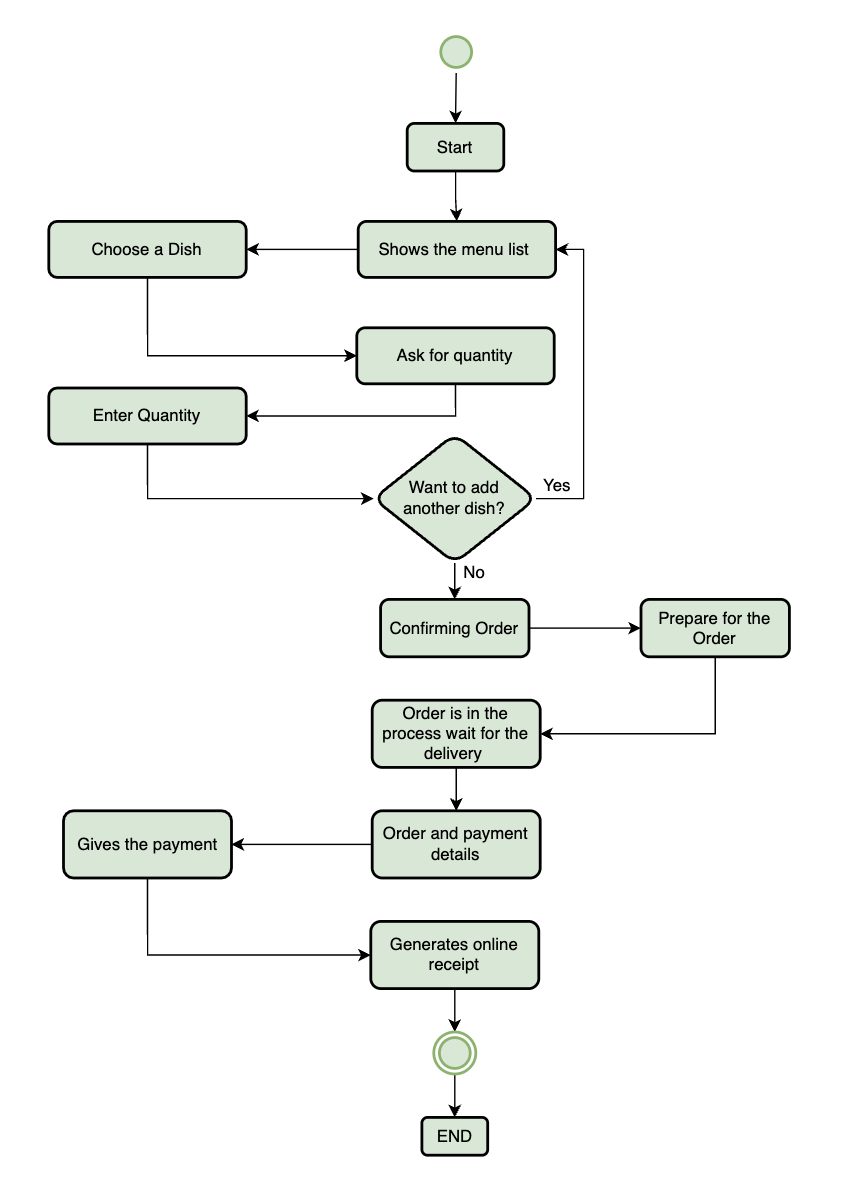
\includegraphics[scale = 0.6]{Activity Diagram 2.png}
\end{center}
\section{\textbf{State Chart Diagram}}
\begin{center}
	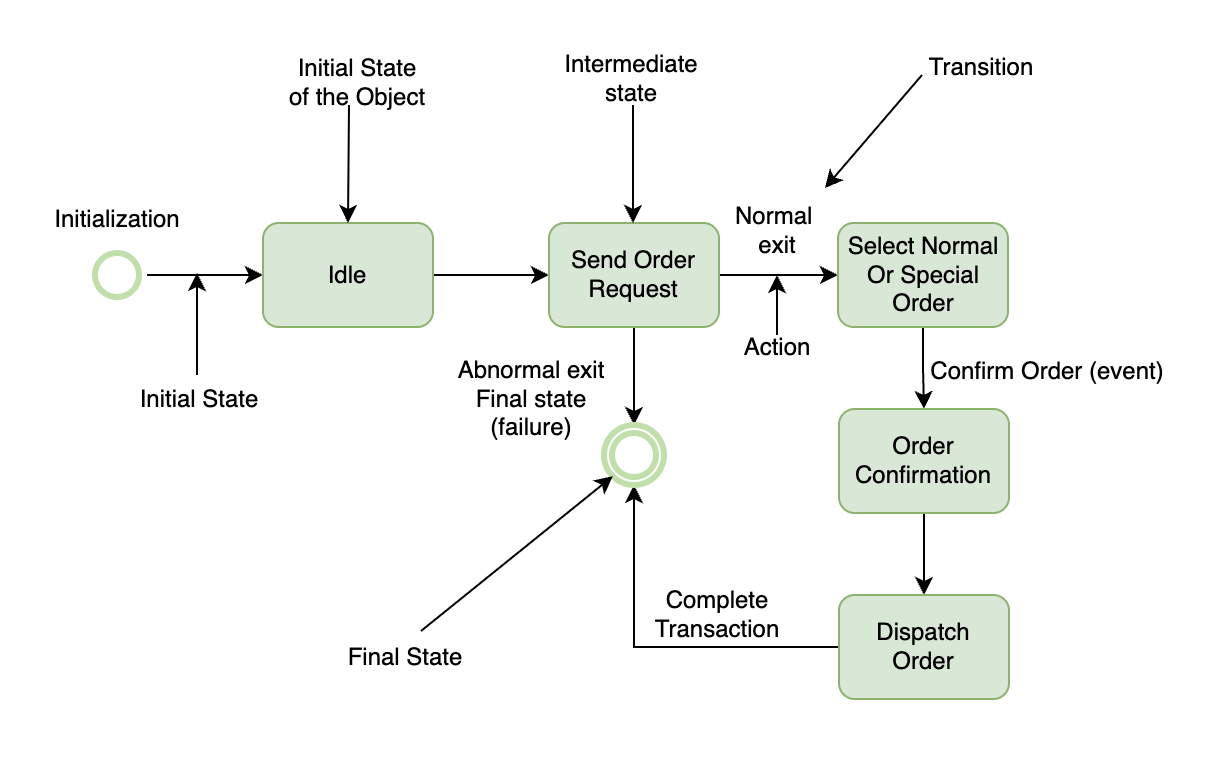
\includegraphics[scale = 0.6]{StateChartDiagram.png}
\end{center}
\section{\textbf{Conclusion}}
Thus, we have studied the Activity Diagram and State Chart Diagram.
\section{\textbf{FAQ's}}
\subsection{\textit{Give the significance of activity diagram.}}
\textbf{Ans.} Activity diagrams are a type of behavioral diagram in UML (Unified Modeling Language) that visually represent the flow of activities or actions within a system, process, or workflow. They are used to model and analyze the steps, decisions, and parallel or sequential flows involved in a particular process. The significance of activity diagrams lies in their ability to:
\begin{enumerate}
	\item Visualize Process Flow: Activity diagrams provide a clear and intuitive visualization of how activities and actions are sequenced and organized within a process. They help stakeholders understand the overall flow and structure of a system or process, including the order of activities, decision points, and branching paths.
	\item Capture Business Processes: Activity diagrams are commonly used to model and analyze complex business processes. They enable business analysts and stakeholders to capture the steps and interactions involved in various business scenarios, such as order processing, customer onboarding, or inventory management. By visually representing the activities and their relationships, activity diagrams facilitate a shared understanding of the process across teams and stakeholders.
	\item Identify Control and Data Flows: Activity diagrams depict the control flow, showing how control passes from one activity to another based on conditions or triggers. They also illustrate the data flow, indicating the movement of data or information between activities. This helps in identifying the dependencies and data requirements within a process and ensures that the necessary inputs are available for each activity.
	\item Analyze Process Behavior: Activity diagrams support the analysis of process behavior by enabling the identification of bottlenecks, inefficiencies, or potential improvements. By examining the sequence of activities and their relationships, stakeholders can identify areas for optimization, resource allocation, or workflow restructuring. This analysis aids in streamlining processes, reducing errors, and improving overall efficiency.
	\item Facilitate Communication and Collaboration: Activity diagrams provide a common visual language for communication and collaboration among stakeholders, including business analysts, developers, and end-users. They serve as a bridge between technical and non-technical stakeholders, allowing for effective communication and understanding of complex processes. Activity diagrams can be used in requirements gathering, system design, and user training to ensure that everyone has a shared understanding of the process flow.
	\item Support System Design and Implementation: Activity diagrams serve as a basis for system design and implementation by providing a blueprint for developers and software engineers. They help in decomposing complex processes into manageable tasks and activities, which can be further refined and implemented as part of the software or system development process. Activity diagrams guide the implementation by illustrating the necessary control structures, decision points, and interactions.
\end{enumerate}
In summary, activity diagrams are valuable tools for modeling, analyzing, and communicating the flow of activities within a process or system. They support process understanding, process improvement, and system design, facilitating effective collaboration and decision-making among stakeholders.
\subsection{\textit{Explain any two terminologies used in activity diagram.}}
\textbf{Ans.} Two terminologies commonly used in activity diagrams:
\begin{enumerate}
	\item Activity: In an activity diagram, an activity represents a specific action or task that occurs within a process. It is a unit of work that can be performed by a system, a user, or a combination of both. Activities are depicted as rounded rectangles with the activity name written inside. They can represent various types of actions, such as calculations, data manipulation, decision-making, or communication with external systems.\\
	Activities can be further decomposed into sub-activities, allowing for a more detailed breakdown of the process. The flow of control moves from one activity to another, indicating the sequence in which the activities are executed. Activities can also have incoming and outgoing edges, representing the control flow from one activity to another.
	\item Decision Node: A decision node, also known as a decision point or diamond shape, represents a point in the process where a decision is made based on certain conditions or criteria. It represents a branching point in the flow of activities, where the process can follow different paths based on the outcome of the decision.\\
	A decision node typically has multiple outgoing edges, each labeled with a condition or a logical expression that determines which path is taken. These conditions are often represented using Boolean expressions or other decision logic. The decision node evaluates the conditions and selects the appropriate outgoing edge to follow, based on the evaluation result.\\
	The decision node allows for modeling of alternative flows and decision-making within a process. It helps in capturing the logic and conditions that govern the behavior of the system or the process being modeled. The decision node is an important construct in activity diagrams as it enables modeling of complex decision-making scenarios and branching paths.
\end{enumerate}
By using these two terminologies, activities and decision nodes, activity diagrams can effectively capture and represent the flow of activities, decision points, and control flow within a process, making them valuable for process modeling and analysis.
\subsection{\textit{Explain the message passing in State Chart Diagram.}}
\textbf{Ans.} In a state chart diagram, message passing represents the communication and interaction between objects or components within a system as they transition between states. It allows objects to exchange information and trigger actions in response to events or conditions. Message passing is a fundamental concept in modeling the dynamic behavior of a system.\\

Here's how message passing works in a state chart diagram:
\begin{enumerate}
	\item Objects: In a state chart diagram, objects are represented by states. Each state represents a specific condition or situation that an object can be in. Objects can be in one state at a time, and they transition from one state to another based on events or conditions.
	\item Events: Events are triggers that cause state transitions in an object. They can be internal or external to the object. Internal events are events that occur within the object itself, such as a timer expiring or a condition being met. External events are events that come from outside the object, such as user inputs or system notifications.
	\item Transitions: Transitions represent the change of state in an object in response to events or conditions. They are depicted as arrows connecting the states. When an event occurs or a condition is met, the object transitions from its current state to a new state. Transitions can have associated actions or activities that are performed during the transition.
	\item Message Passing: Message passing occurs when an object sends a message to another object, typically as part of a state transition. The message contains information or a command that is intended for the receiving object. It can trigger an action in the receiving object or provide data for processing.
	\item Actions and Behaviors: Actions are the operations or behaviors performed by objects in response to events or messages. When an object receives a message, it can execute a specific action or behavior associated with that message. This could involve changing internal variables, invoking methods, or interacting with other objects or components.
\end{enumerate}
Message passing allows objects to communicate and collaborate in a system, enabling the exchange of information and coordination of activities. It models the interactions and dependencies between objects as they transition between states. By specifying the messages and actions associated with transitions, state chart diagrams provide a clear representation of the dynamic behavior and message flow within a system.\\

Overall, message passing in state chart diagrams facilitates the modeling and analysis of the communication and interaction patterns between objects, helping to design and understand the behavior of complex systems.
\end{document}